\section{Introduction}

\frame{
	\frametitle{Current Gen Attribute Grammars}
    
	\begin{itemize}
	\item<1-> Computations over a single tree
    \item<2-> Function over attributes
    \item<3-> Visits are implicit
	\item<4-> Same phase for synthesis and evaluation
	\item<5-> Can describe inference but not unification
	\end{itemize}
}

\frame{
	\frametitle{Next Gen Attribute Grammars}
    
	\begin{itemize}
	\item<1-> Allows Computations over multiple trees
	\item<2-> Based on visit sequences
    \item<3-> Supports explicit visits
    \item<4-> Supports multiple visits
    \item<5-> Separate phases for synthesis and evaluation
	\end{itemize}
}

\frame{
	\frametitle{Why Attribute Grammars}
    
	Implement type system using attribute grammars
	\begin{itemize}
	\item<1-> Easier to understand
	\item<2-> Easier to prove correct
	\item<3-> Easier to document and scale
	\end{itemize}
}

\section{Ruler-core}

\frame{
	\frametitle{Ruler-Core}
	
    \begin{block}<+->{Developed by Arie Middelkoop}
	\begin{definition}
		A programming language to manipulate visit sequences
	\end{definition}
    \end{block}
}

\frame{
	\frametitle{Ruler-Core}
	
	\begin{block}<+->{visits}
	\begin{itemize}
	\item<1-> A (partial) function
    \item<2-> Takes several inputs (inherited)
	\item<3-> Produces several outputs (synthesized)
	\item<4-> A continuation for the next visit.
	\end{itemize}
	\end{block}
}

\frame{
	\frametitle{A case study}
	
	Implementing the Hindley-Milner type system
}

\frame{
	\frametitle{Hindley-Milner}
    
	\begin{itemize}
	\item<1-> Damas-Milner
	\item<2-> Principle type
	\item<3-> Build set of constrains
	\item<4-> Decidable inferencing
	\end{itemize}
}

\frame{
	\frametitle{Datatypes: TyExpr}
	
	\begin{columns}
		\begin{column}[c]{0.5\linewidth}
		\begin{code}
           data TyExpr
             con Var
                 nm      ::  Name
             con Con        
                 nm      ::  Name
             con App        
                 func    :  TyExpr
                 arg     :  TyExpr
             con Paren      
                 tyExpr  :  TyExpr
		\end{code}
		\end{column}
		\begin{column}[c]{0.5\linewidth}
		\begin{description}
		\item[|:|]  are terminals
		\item[|::|] are nonterminals
		\end{description}
		\end{column}
	\end{columns}
}

\frame{
	\frametitle{Datatypes: Expr}
	
	\begin{columns}
	\begin{column}[t]{0.5\linewidth}
	\begin{code}
    data Expr 
        con IConst
            int    ::  Int
        con Var       
            nm     ::  Name
        con Con       
            nm     ::  Name
        con Lam       
            arg    ::  Name
            body   :  Expr
	\end{code}
	\end{column}
	\begin{column}[t]{0.5\linewidth}
	\begin{code}
    con App   
       func    :  Expr
       arg     :  Expr
    con Let       
       nm      ::  Name
       bind    :  Expr
       body    :  Expr
    con Paren     
       tyExpr  :  Expr
	\end{code}
	\end{column}
	\end{columns}
}

\frame{
	\frametitle{interfaces}
	
	\begin{columns}
	\begin{column}[c]{0.4\linewidth}
	\begin{code}
    itf <name>
      {visit <name>
        {attributes}
      }
    \end{code}
	\end{column}
	\begin{column}[c]{0.6\linewidth}
	\begin{itemize}
	\item<1-> Declare nonterminals
	\item<2-> Multiple visits
	\item<3-> Every visit is a co-routine
	\item<4-> order is not relevant
	\item<5-> Will be automatically scheduled
	\end{itemize}
	\end{column}
	\end{columns}
}

\frame{
	\frametitle{Inference interface}
	
	\begin{columns}
	\begin{column}[c]{0.4\linewidth}
    \begin{code}
    	itf Expr
          visit infer
            inh ast  ::  Expr
            inh env  ::  Gamma
            inh frs  ::  Int
            syn frs  ::  Int
            syn sub  ::  Env
            syn ty   ::  TyExpr
    \end{code}
	\end{column}
	\begin{column}[c]{0.6\linewidth}
	\begin{description}
	\item[inh] inherited attributes
	\item[syn] synthesized attributes
	\item[] Attributes can share names
    \item[ast] reguired attribute
	\end{description}
	\end{column}
	\end{columns}
}

\frame{
    \frametitle{Semantics}
    
	\begin{block}<+->{There are two kinds of visits}
	\begin{itemize}
	\item<1->{Declared inside of interfaces
        \begin{itemize}
        \item<2-> Declares what to calculate
        \end{itemize}
        }
    \item<3->{Declared inside of semantic functions
        \begin{itemize}
        \item<4-> Declares how to calculate
        \end{itemize}
        }
	\end{itemize}
	\end{block}
}

\frame{
	\frametitle{Semantic functions}
	
	\begin{itemize}
	\item datasem (datatype semantic functions)
	\item sem (semantic function for an arbitrary interface)
	\end{itemize}
}

\frame{
    \frametitle{Datasem}
    
    \begin{code}
    datasem <nonterminal> 
        {clause <name>
            ...
        }
    \end{code}
    
    \begin{itemize}
    \item<1-> Declares semantics for a nonterminal
    \item<2-> Clauses correspond to constructors
    \item<3-> Implicit children for nonterminals
    \end{itemize}
}

\frame{
    \frametitle{Clauses}
    
    \begin{code}
    clause <ident>
      { rules }
    \end{code}
    
    \begin{itemize}
    \item<1-> Provide a means of scoping
    \item<2-> A way to do alternatives
    \item<3-> Tried sequentially
    \item<4-> Backtracks if not applicable
    \item<5-> contain rules (matches, bindings etc)
    \end{itemize}
}

\frame{
    \frametitle{Defining inference}
    
    \begin{code}
    datasem Expr monad IO
        clause IConst
          lhs.ty   =  TyExpr_Con "Int"
          lhs.sub  =  []
          lhs.frs  =  lhs.frs
    \end{code}
}

\frame{
    \frametitle{Defining inference}
    
    \begin{code}
    datasem Expr monad IO
        clause IConst
          lhs.ty   =  TyExpr_Con "Int"
          lhs.sub  =  []
          lhs.frs  =  lhs.frs
        clause Var   
          lhs.ty   =  fromMaybe (error ...) (lookup loc.nm lhs.env)
          lhs.sub  =  []
          lhs.frs  =  lhs.frs
    \end{code}
}

\frame{
    \frametitle{Defining inference}
    
    \begin{code}
    datasem Expr monad IO
        clause IConst
          lhs.ty   =  TyExpr_Con "Int"
          lhs.sub  =  []
          lhs.frs  =  lhs.frs
        clause Var   
          lhs.ty   =  fromMaybe (error ...) (lookup loc.nm lhs.env)
          lhs.sub  =  []
          lhs.frs  =  lhs.frs
        clause Con   
          lhs.ty   =  TfromMaybe (error ...) (lookup loc.nm lhs.env)
          lhs.sub  =  []
          lhs.frs  =  lhs.frs
    \end{code}
}

\frame{
    \frametitle{Defining inference}
    
    \begin{code}
    datasem Expr monad IO
        clause IConst
          lhs.ty   =  TyExpr_Con "Int"
          lhs.sub  =  []
          lhs.frs  =  lhs.frs
        clause Var   
          lhs.ty   =  fromMaybe (error ...) (lookup loc.nm lhs.env)
          lhs.sub  =  []
          lhs.frs  =  lhs.frs
        clause Con   
          lhs.ty   =  fromMaybe (error ...) (lookup loc.nm lhs.env)
          lhs.sub  =  []
          lhs.frs  =  lhs.frs
        clause Paren
          tyExpr.frs  =  lhs.frs
          lhs.ty      =  tyExpr.ty
          lhs.sub     =  tyExpr.sub
    \end{code}
}

\frame{
    \frametitle{Defining inference}
    
    \begin{code}
    datasem Expr monad IO
        default? frs  =  last
        default? sub  =  last
        default? env  =  last
        clause IConst
          lhs.ty   =  TyExpr_Con "Int"
          lhs.sub  =  []
        clause Var   
          lhs.ty   =  fromMaybe (error ...) (lookup loc.nm lhs.env)
          lhs.sub  =  []
        clause Con   
          lhs.ty   =  fromMaybe (error ...) (lookup loc.nm lhs.env)
          lhs.sub  =  []
        clause Paren
          lhs.ty  =  tyExpr.ty
    \end{code}
}

\frame{
    \frametitle{Default rules}
    
    \textbf{default[\textit{?}]} \hspace{5pt} \emph{attribute} = \emph{function}
        
	\begin{block}<+->{defining default values for attributes}
		\begin{description}
        \item[] Collect |attribute| values in a list
		\item[default] throws static exception
        \item[default?] returns empty list
		\end{description}
	\end{block}
}

\frame{
    \frametitle{Default rules}
    \center
    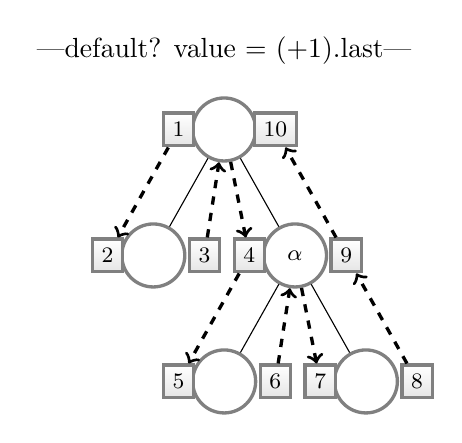
\begin{tikzpicture}
    [ nd/.style={circle, minimum size=8mm, very thick, draw=black!50!black!50, top color=white, bottom color=white,font=\footnotesize}
    , attr/.style={rectangle, minimum size=1mm, node distance=4mm, very thick, draw=black!50, top color=white, bottom color=gray!20,font=\footnotesize}
    , inh/.style={attr}
    , inh1/.style={syn, xshift=-1.8mm}
    , syn/.style={attr}
    , syn1/.style={syn, xshift=2.5mm}
    , syn2/.style={syn, xshift=4mm}
    , syn3/.style={syn, xshift=1mm, yshift=-3mm}
    , arr/.style={->,dashed, very thick}
    ]
    
    \node[nd](n1){}
      [sibling distance=18mm, level distance=16mm]
      child {
        node[nd](n2){}
      }
      child {
        node[nd](n3){$\alpha$}
          child {
            node[nd](n4){}
          }
          child {
            node[nd](n5){}
          }
      };
      
    \node[syn1, right of=n1] (n1syn) {10};
    \node[syn1, right of=n2] (n2syn) {3};
    \node[syn1, right of=n3] (n3syn) {9};
    \node[syn1, right of=n4] (n4syn) {6};
    \node[syn1, right of=n5] (n5syn) {8};
      
    \node[inh1, left of=n1] (n1inh) {1};
    \node[inh1, left of=n2] (n2inh) {2};
    \node[inh1, left of=n3] (n3inh) {4};
    \node[inh1, left of=n4] (n4inh) {5};
    \node[inh1, left of=n5] (n5inh) {7};
    
	\node[above of=n1]{|default? value = (+1).last|};

    \draw[arr] (n1inh) to (n2inh);
    \draw[arr] (n2syn) to (n1);
    \draw[arr] (n1)    to (n3inh);
    \draw[arr] (n3inh) to (n4inh);
    \draw[arr] (n4syn) to (n3);
    \draw[arr] (n3)    to (n5inh);
    \draw[arr] (n5syn) to (n3syn);
    \draw[arr] (n3syn) to (n1syn);
    
    \end{tikzpicture}
    
    $\alpha = [1,2,3,4]$
}

\frame{
    \frametitle{Defining inference}
    
    \begin{prooftree}
		\AxiomC{$\Gamma \vdash x : \tau_1 \quad e : \tau_2$}
	\LeftLabel{Lam:\quad}
		\UnaryInfC{$\Gamma \vdash \lambda x \rightarrow e : \tau_1 \rightarrow \tau_2$}
\end{prooftree}
    
    \begin{code}
    clause Lam
      (loc.a, loc.frs) = first TyExpr_Var (fresh lhs.frs)
      body.env  =  (loc.arg, loc.a):lhs.env
      body.frs  =  loc.frs
      
      lhs.ty    =  (appAll body.sub loc.a) `mkArrow` body.ty
    \end{code}
}

\frame{
    \frametitle{Defining inference}
    
    \begin{prooftree}
		\AxiomC{$\Gamma \vdash f : \tau_1 \rightarrow \tau_2 \quad x : \tau_1$}
	\LeftLabel{App:\quad}
		\UnaryInfC{$\Gamma \vdash f \hspace{3pt} x : \tau_2$}
\end{prooftree}
    
    \begin{code}
    clause App
      (loc.b, loc.frs) = first TyExpr_Var (fresh lhs.frs)
      
      func.frs  =  loc.frs
      arg.frs   =  func.frs
    \end{code}
}

\frame{
    \frametitle{Defining inference}
    
    \begin{prooftree}
		\AxiomC{$\Gamma \vdash f : \tau_1 \rightarrow \tau_2 \quad x : \tau_1$}
	\LeftLabel{App:\quad}
		\UnaryInfC{$\Gamma \vdash f \hspace{3pt} x : \tau_2$}
\end{prooftree}
    
    \begin{code}
    clause App
      (loc.b, loc.frs) = first TyExpr_Var (fresh lhs.frs)
      
      func.frs  =  loc.frs
      arg.frs   =  func.frs
      
      child u : Unify = unify
      u.frs   =  arg.frs
      u.exp1  =  func.ty
      u.exp2  =  arg.ty `mkArrow` loc.b
    \end{code}
}

\frame{
    \frametitle{Defining inference}
    
    \begin{prooftree}
		\AxiomC{$\Gamma \vdash f : \tau_1 \rightarrow \tau_2 \quad x : \tau_1$}
	\LeftLabel{App:\quad}
		\UnaryInfC{$\Gamma \vdash f \hspace{3pt} x : \tau_2$}
\end{prooftree}
    
    \begin{code}
    clause App
      (loc.b, loc.frs) = first TyExpr_Var (fresh lhs.frs)
      
      func.frs  =  loc.frs
      arg.frs   =  func.frs
      
      child u : Unify = unify
      u.frs   =  arg.frs
      u.exp1  =  func.ty
      u.exp2  =  arg.ty `mkArrow` loc.b
      
      lhs.ty   =  appAll u.sub loc.b
      lhs.sub  =  func.sub ++ arg.sub ++ u.sub
      lhs.frs  =  u.frs
    \end{code}
}

\frame{
    \frametitle{Child}
    
    \textbf{child} \hspace{5pt} \emph{name} : Interface \hspace{5pt} [= sem\_name]
    
    \begin{itemize}
    \item Declares a new \textbf{child} \emph{name}
    \item Of nonterminal Interface
    \item sem\_name by default |id|
    \end{itemize}
}

\frame{
    \frametitle{Defining inference}
    
    \begin{prooftree}
		\AxiomC{$\Gamma \vdash e_1 : \tau_1 \quad (\Gamma, x : \tau_1) \vdash e_2 : \tau_2 $}
	\LeftLabel{Let:\quad}
		\UnaryInfC{$\Gamma \vdash Let \hspace{3pt} x = e_1 \hspace{3pt} in \hspace{3pt} e_2 : \tau_2$}
\end{prooftree}
    
    \begin{code}
    clause Let
      body.env  =  (loc.nm, bind.ty):lhs.env
      lhs.ty    =  body.ty
    \end{code}
}

\frame{
    \frametitle{Unification}
    
    \begin{code}
    itf Unify
      visit unify
        inh exp1  ::  TyExpr
        inh exp2  ::  TyExpr
        inh frs   ::  Int
        syn sub   ::  Env
        syn frs   ::  Int
    \end{code}
    
    \begin{itemize}
    \item Unification requires traversal of two trees
    \item Unify |exp1| with |exp2|
    \end{itemize}
}

\frame{
    \frametitle{Semantic function}
    
    \begin{code}
    <name> = sem <internal_name> : <Interface>
              {visit <name>
                 {clause <name>
                    ...
                 }
              }
    \end{code}
    
    \begin{itemize}
    \item defines semantic function for arbitrary interface
    \end{itemize}
}

\frame{
    \frametitle{Unification}
    
    \begin{code}
    unify = sem unify : Unify monad IO
          visit unify
            default? frs  =  last
            default? sub  =  const []
            clause LeftParen
              match TyExpr.Paren@exp1 = lhs.exp1
              
              child u : Unify = unify
              
              u.exp1  = exp1.tyExpr
              u.exp2  = lhs.exp2
    \end{code}
    
    \begin{itemize}
    \item Physical parenthesis can be removed
    \item Identical case for the right parenthesis
    \end{itemize}
}

\frame{
    \frametitle{Match}
    
    \begin{code}
    match TypeName.ConstructorName@child  = <expression>
    \end{code}
    
    \begin{itemize}
    \item |var| and |lhs| are restricted keywords
    \item Build in types such as |Bool| are special
    \item<2-> |match True = ...|
    \end{itemize}
}

\frame{
    \frametitle{Unification}
    
    \begin{code}
     clause constructor
          match TyExpr.Con@exp1  =  lhs.exp1
          match TyExpr.Con@exp2  =  lhs.exp2
          
          lhs.sub = case exp1.nm == exp1.nm of
                      True   ->  []
                      False  ->  error ...
    \end{code}
    
}

\frame{
    \frametitle{Unification}
    
    \begin{code}
     clause app
          match TyExpr.App@app1  =  lhs.exp1
          match TyExpr.App@app2  =  lhs.exp2  
          
          child u1 : Unify = unify
          
          u1.exp1  =  app1.func
          u1.exp2  =  app2.func
    \end{code}
}

\frame{
    \frametitle{Unification}
    
    \begin{code}
     clause app
          match TyExpr.App@app1  =  lhs.exp1
          match TyExpr.App@app2  =  lhs.exp2  
          
          child u1 : Unify = unify
          
          u1.exp1  =  app1.func
          u1.exp2  =  app2.func
          
          child u2 : Unify = unify
          
          u2.exp1  =  appAll u1.sub app1.arg
          u2.exp2  =  appAll u1.sub app2.arg
                     
          lhs.sub  =  u1.sub ++ u2.sub
    \end{code}
}

\frame{
    \frametitle{Unification}
    
    \begin{code}
    clause vars
      match TyExpr.Var@var1  =  lhs.exp1
      match TyExpr.Var@var2  =  lhs.exp2 
      match True             =  var1.nm == var2.nm
    \end{code}
}

\frame{
    \frametitle{Unification}
    
    \begin{code}
    clause vars
      match TyExpr.Var@var1  =  lhs.exp1
      match TyExpr.Var@var2  =  lhs.exp2 
      match True             =  var1.nm == var2.nm
    clause leftvar
      match TyExpr.Var@var1  =  lhs.exp1
      lhs.sub = [(var1.nm, lhs.exp2)]
    \end{code}
}

\frame{
    \frametitle{Unification}
    
    \begin{code}
    clause vars
      match TyExpr.Var@var1  =  lhs.exp1
      match TyExpr.Var@var2  =  lhs.exp2 
      match True             =  var1.nm == var2.nm
    clause leftvar
      match TyExpr.Var@var1  = lhs.exp1
      lhs.sub = [(var1.nm, lhs.exp2)]
    clause rightvar
      match TyExpr.Var@var1  = lhs.exp2
      lhs.sub = [(var1.nm, lhs.exp1)]
    \end{code}
}

\frame{
    \frametitle{Unification}
    
    \begin{code}
    clause vars
      match TyExpr.Var@var1  =  lhs.exp1
      match TyExpr.Var@var2  =  lhs.exp2 
      match True             =  var1.nm == var2.nm
    clause leftvar
      match TyExpr.Var@var1  =  lhs.exp1
      lhs.sub = [(var1.nm, lhs.exp2)]
    clause rightvar
      match TyExpr.Var@var1  =  lhs.exp2
      lhs.sub = [(var1.nm, lhs.exp1)]
    clause rest
      lhs.sub = error "mismatch in unify."
    \end{code}
}

\frame{
    \frametitle{Invoking function}
    
    \begin{code}
    typeCheck :: Expr -> IO TyExpr
    typeCheck exp = do
      let inh = Inh_Expr_infer
                  { ast_Inh_Expr  =  exp
                  , env_Inh_Expr  =  []
                  , frs_Inh_Expr  =  0
                  }
      syn <- invoke_Expr_infer dnt_Expr inh
      let x = ty_Syn_Expr syn
      return (alpha_rename x)
    \end{code}
}

\frame{
    \frametitle{Results}
    
    \begin{code}
    *HM> let compose = (Expr_Lam "f" ...)
    *HM> compose
    \f -> \g -> \x -> f g x
    *HM> typeCheck compose
    (a4 -> a3) -> (a2 -> a4) -> a2 -> a3
    \end{code}
}

\section{First class polymorphism}
\frame{
	\frametitle{Higher-rank types}
    
	\begin{itemize}
    \item<1-> Haskell '98 types are rank-1
    \item<2-> |a -> b -> a|
    \item<3-> |forall a b. a -> b -> a|
    \item<4-> |forall a. a -> (forall b. b -> a)|
    \item<5-> |forall b. (forall a. a -> a) -> b -> b|
	\end{itemize}

	\only<6->{Refers to the the number of |forall|s nested to the left of a |(->)|}
}

\frame{
	\frametitle{Higher-rank types}
    
	\begin{code}
	poly = \f -> (f 1, f 'c')
	\end{code}
	
	cannot be expressed without Higher-Rank types.
}

\frame{
	\frametitle{SystemF}
   Provides typing support for higher-rank functions

	\begin{block}<+->{Terms}
		\begin{itemize}
		\item Type abstraction ($\Lambda X. t$)
		\item Type application (t [T])
		\end{itemize}
	\end{block}

	\begin{block}<+->{Types}
		\begin{itemize}
		\item Type variables (X)
		\item Universal types (|forall X. T|)
		\end{itemize}
	\end{block}
}

\frame{
	\frametitle{SystemF}
   Typing of the |id| function
	\begin{itemize}
	\item<1-> $id = \lambda x. x$
	\item<2-> $id = \Lambda X. \lambda x : X \rightarrow x : X$
	\item<3-> Typing |id 3|
	\item<4-> id [Int] = [X$\rightarrow$Int]($\lambda x:X. x$)
	\end{itemize}
}

\frame{
	\frametitle{SystemF}
	\begin{itemize}
	\item<1->|poly = \f -> (f 1, f 'c')| is not typeable
	\item<2->Undecidable
	\item<3->Requires annotation
	\item<4->|poly = \(f :: forall a -> Int) -> (f 1, f 'c')|
	\end{itemize}
}

\section{HML}

\frame{
    \frametitle{Introduction}
    
    \begin{itemize}
    \item<1-> Extension of Hindley-Milner
    \item<2-> Supports first class polymorphism
    \item<3-> Insensitive to order of applications
    \end{itemize}
}

\frame{
    \frametitle{Type scheme}
    
    \begin{eqnarray*}
    \varphi & ::= & \forall (\alpha \geq \varphi_1). \varphi_2 \\
            & || & \sigma \\
            & || & \bot
    \end{eqnarray*}
    
    \begin{description}
    \item[trivial] $\forall (\alpha \geq Int). \varphi$
    \item[unconstrained] $\forall (\alpha \geq \bot). \varphi$
    \end{description}
}

\frame{
    \frametitle{Type Prefix}
    
    \begin{eqnarray*}
    Q ::= \alpha_1\geq\hat{\varphi}_1,\ldots,\alpha_n\geq\hat{\varphi}_n
    \end{eqnarray*}
    
    \begin{itemize}
    \item<1-> Cannot contain a trivial bounds
    \item<2-> domain of prefix and substitutions disjoint
    \item<3-> A type is quantified by prefix or itself
    \end{itemize}
}

\frame{
    \frametitle{Benefits}
    
    \begin{quotation}
    \textit{inc} $\hspace{16.5pt}$ :: Int $\rightarrow$ Int\\
    \indent \textit{single} $\hspace{3pt}$  :: $\forall\alpha$. $\alpha$ $\rightarrow$ List $\alpha$\\
    \indent \textit{append}  :: $\forall\alpha$. List $\alpha$ $\rightarrow$ List $\alpha$ $\rightarrow$ List $\alpha$\\
    \indent \textit{map} $\hspace{10.2pt}$  :: $\forall\alpha\beta$. ($\alpha$ $\rightarrow$ $\beta$) $\rightarrow$ List $\alpha$ $\rightarrow$ List $\beta$ 
    \end{quotation}
    
    and the expression
    
     \begin{code}
    let ids   =  single id
        poly  =  \(f::forall a. a -> a) -> (f 1, f 'a')
    in  (map poly ids, append (single inc) ids)
    \end{code}
}

\frame{
    \frametitle{Benefits}
    
    \begin{code}
    let ids   =  single id
        poly  =  \(f::forall a. a -> a) -> (f 1, f 'a')
    in  (map poly ids, append (single inc) ids)
    \end{code}
    
    \begin{itemize}
    \item<1-> Not possible in GHC
    \item<2-> Requires |ids| to be List (Int $\rightarrow$ Int) and List ($\forall\alpha$. $\alpha$ $\rightarrow$ $\alpha$)
    \item<3-> Anything inside the bounds are instantiated
    \item<4-> |forall(beta >= forall alpha. alpha -> alpha) . List beta|
    \item<5-> "The type |List beta| can be used for any |beta| that is an instance of |forall alpha. alpha -> alpha|"
    \end{itemize}
}

\section{Conclusion}

\frame{
    \frametitle{Conclusions}
    
    \begin{itemize}
    \item Ruler-core allows traversals of arbitrary number of trees
    \item Default rules save a lot of work
    \item Higher-ordered
    \item Saved \~26\% of code on case study
    \end{itemize}
}
